\section{Ultra Accuracy (UAC)}

	\subsection{UAC-Bondhead 2 (BH)}
		Dies ist ein rework des UAV-BH 1, dabei ist das Luftlagerlager von Eitzenberger und die Vakuumzuführung auf Besi-Seite verbessert worden.
		\begin{figure}[h!]
			\centering
			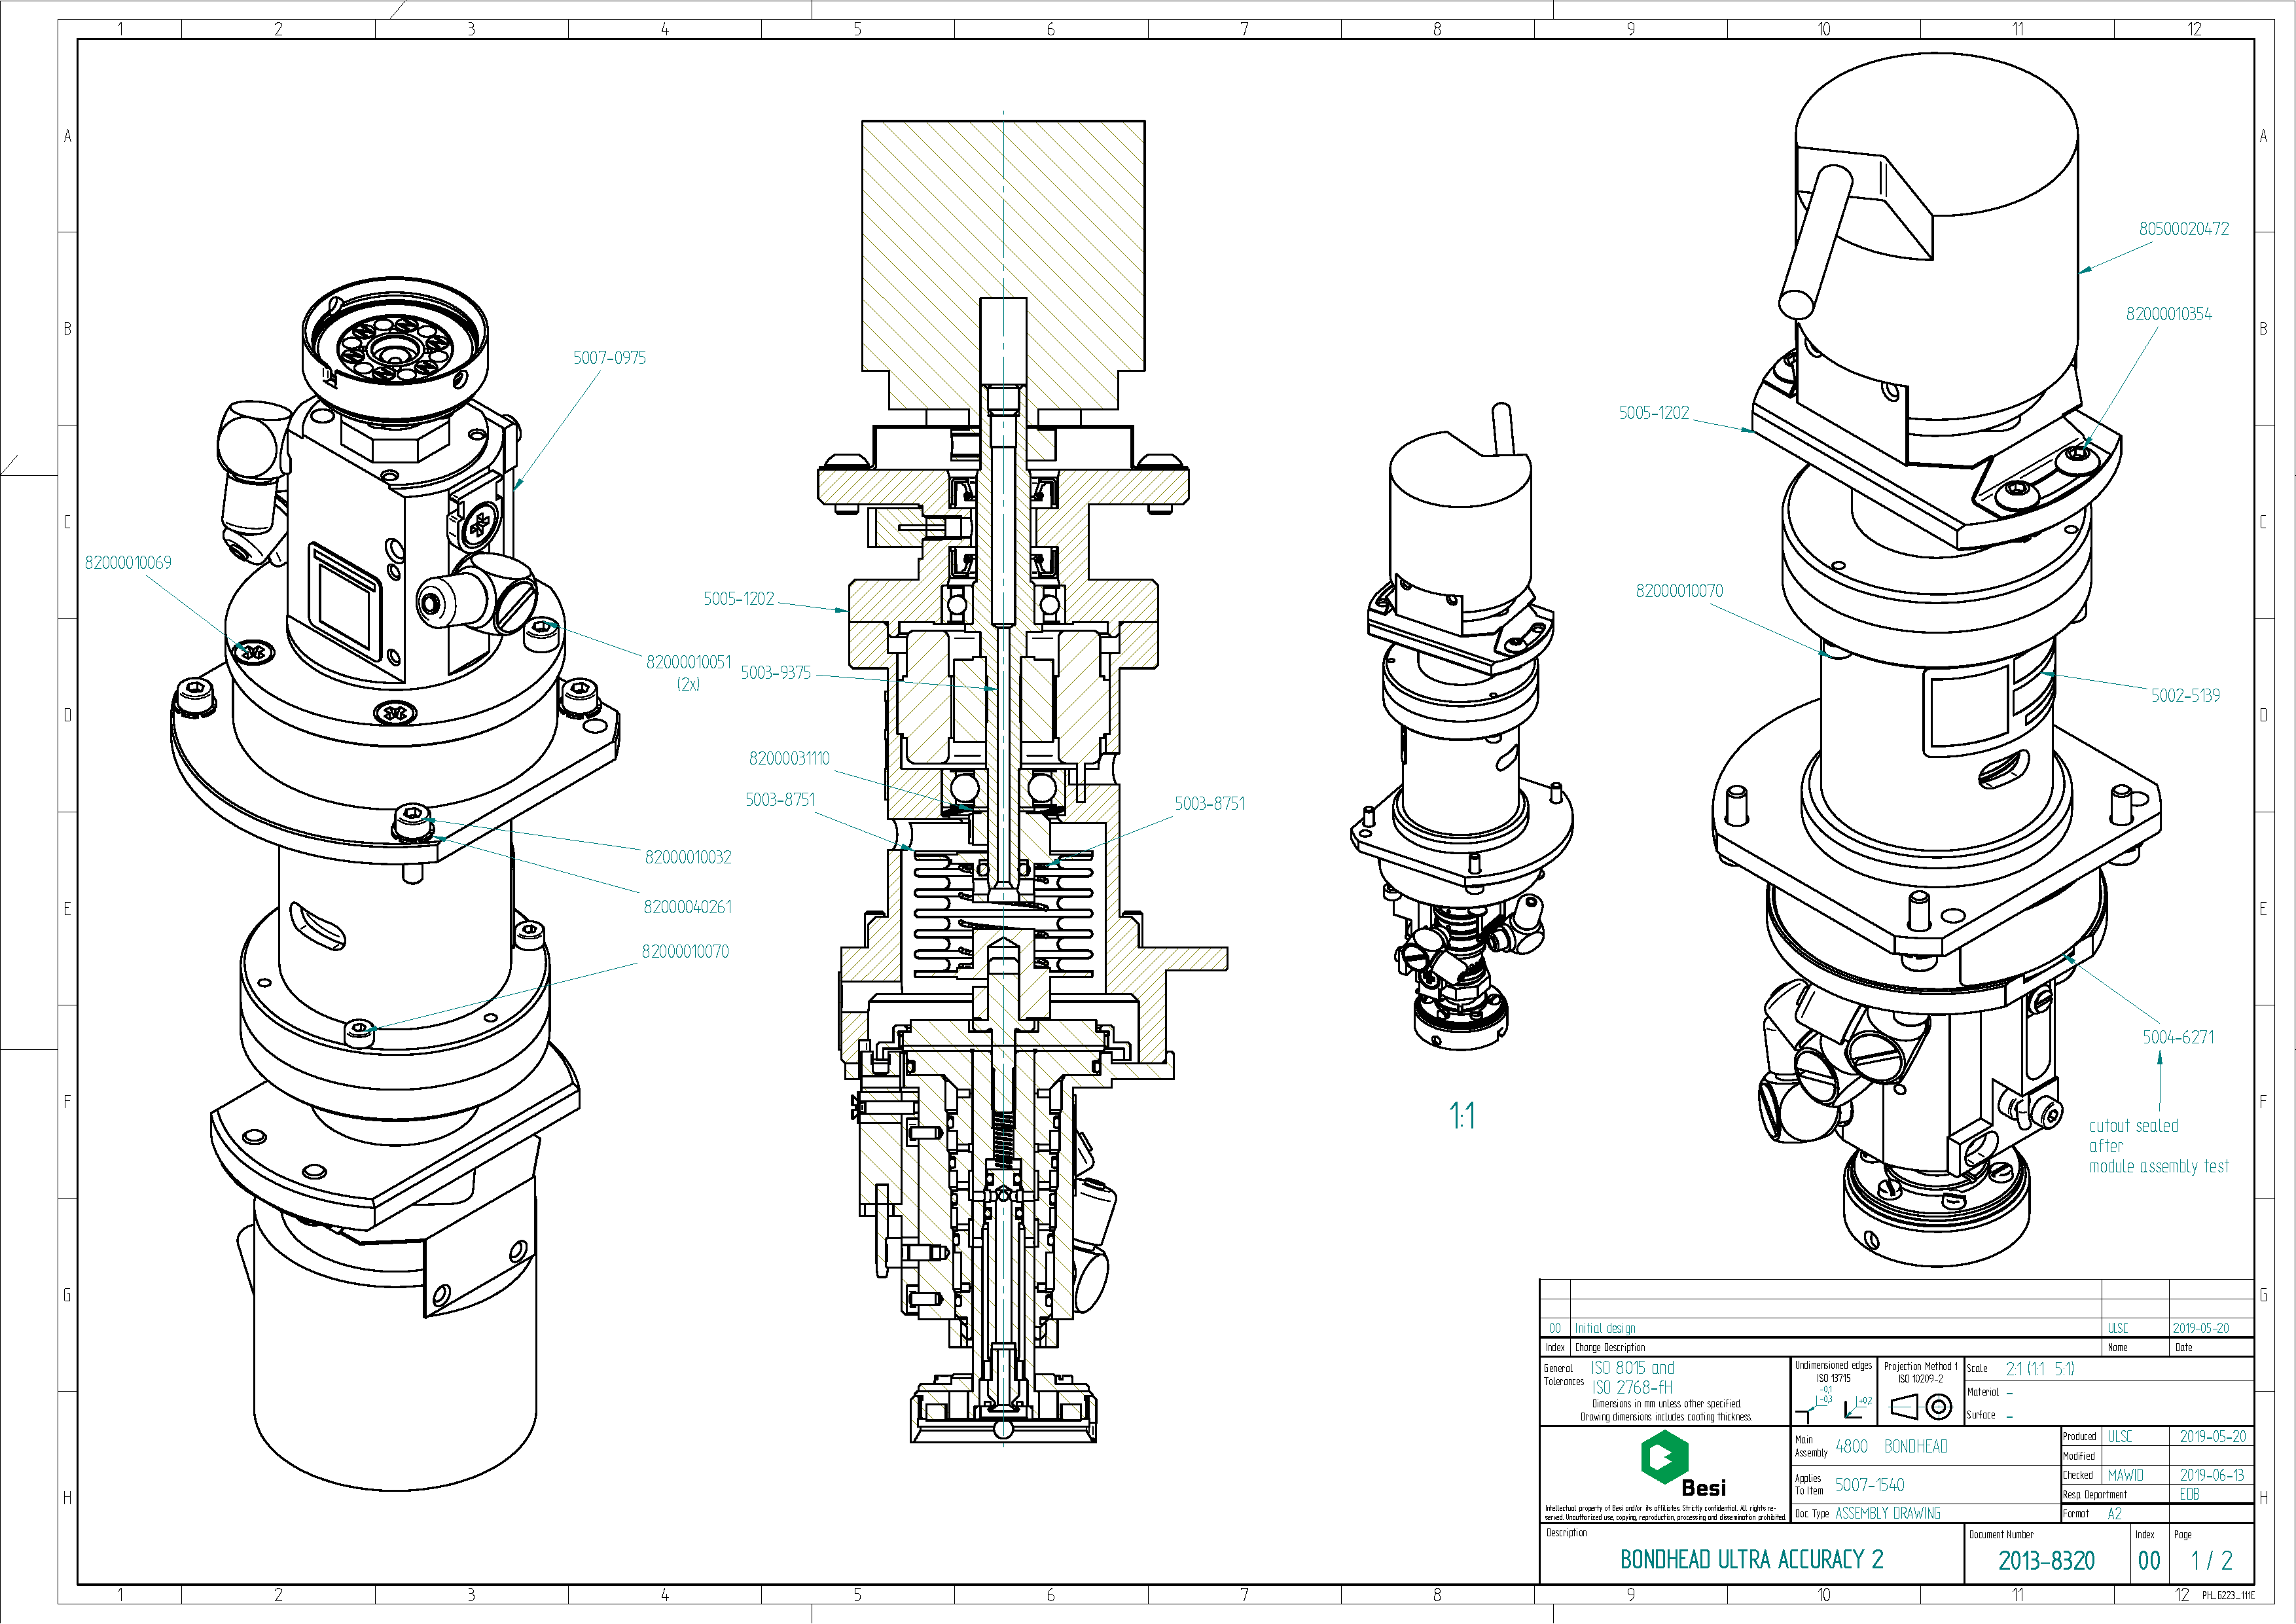
\includegraphics[width=0.999\linewidth]{./pics/UAC/UAC_Bondhead2.pdf}
		\end{figure}
		\begin{figure}[h!]
			\centering
			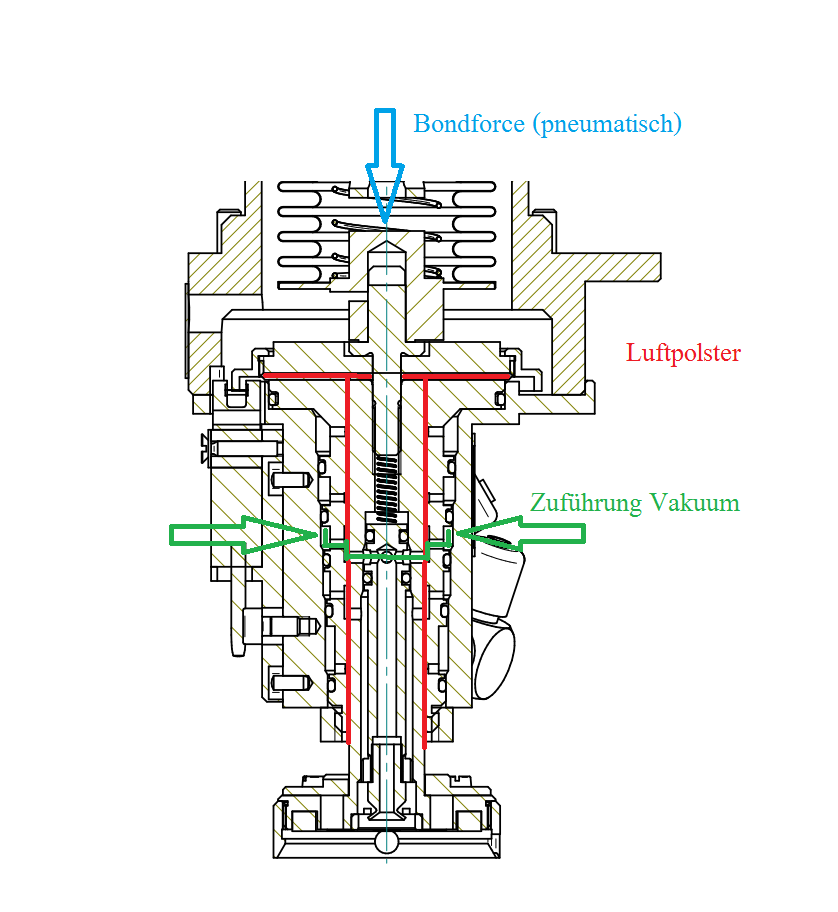
\includegraphics[width=\linewidth]{./pics/UAC/pneu.png}
		\end{figure}
		Durch den pneumatischen Druck in der Druckdose wird die Scheibe (des luftgelagerten Teils) erst nach unten gedrückt und es kann sich erst dann das horizontale Luftpolster in Axialrichtung bilden. Der Druck in der Druckdose bestimmt zugleich die Bondforce. Denn wird der Anpressdruck durch die z-Achse größer als jene Kraft durch die Druckdose verursacht, dann hebt sich die Scheibe wieder und es wird eine Lichtschranke betätigt. Das triggert ein Event und der nächste Prozessschritt wird ausgelöst.